%% LaTeX Beamer presentation template (requires beamer package)
%% see http://latex-beamer.sourceforge.net/
%% idea contributed by H. Turgut Uyar
%% template based on a template by Till Tantau
%% this template is still evolving - it might differ in future releases!

\documentclass[13pt]{beamer}

% \mode<presentation>
% {
% \usetheme{Warsaw}
% 
% \setbeamercovered{transparent}
% }
\usepackage[english]{babel}
\usepackage[latin1]{inputenc}

% font definitions, try \usepackage{ae} instead of the following
% three lines if you don't like this look
\usepackage{mathptmx}
\usepackage[scaled=.90]{helvet}
\usepackage{courier} 

\usepackage{graphicx}

\usepackage[T1]{fontenc}

\beamertemplatetransparentcoveredhigh

\def\hilite<#1>{%
\temporal<#1>{\color{gray}}{\color{black}}%
{\color{gray}}}
 
\title{Towards a Crosscutting Approach for Variability Management}
% \subtitle{SPLC Doctoral Symposium}


% - Use the \inst{?} command only if the authors have different
%   affiliation.
%\author{F.~Author\inst{1} \and S.~Another\inst{2}}
\author{Rodrigo Bonif\'{a}cio \and Paulo Borba}

% - Use the \inst command only if there are several affiliations.
% - Keep it simple, no one is interested in your street address.
\institute
{
	Informatics Center \\ Federal University of Pernambuco \\ Brazil
}

% \date{\date() / SPLC Doctoral Symposium}


% This is only inserted into the PDF information catalog. Can be left
% out.
%\subject{Talks}



% If you have a file called "university-logo-filename.xxx", where xxx
% is a graphic format that can be processed by latex or pdflatex,
% resp., then you can add a logo as follows:

% \pgfdeclareimage[height=0.5cm]{university-logo}{university-logo-filename}
% \logo{\pgfuseimage{university-logo}}




% If you wish to uncover everything in a step-wise fashion, uncomment
% the following command:

%\beamerdefaultoverlayspecification{<+->}

\begin{document}

\begin{frame}
\titlepage
\end{frame}

\section{Introduction}

\begin{frame}
\frametitle{Software Product Line (SPL)}

\begin{block}{Definition}
\begin{itemize}
  \item The SPL approach is a well known technique for implementing systematic
  reuse in software engineering.
  \item Based on this approach, products are customized (or generated) from a
  set of reusable assets.
\end{itemize}
\end{block}
\end{frame}

\begin{frame}
\frametitle{Software Product Line (SPL)}

\begin{block}{Technical point: variability management}
\begin{itemize}
  \item Reusable assets are extensible by means of variation points.
  \item Different techniques might be used to solve these VPs.
  \item Product decisions (capabilities) drive the generation process.
\end{itemize}
\end{block}

\center{
 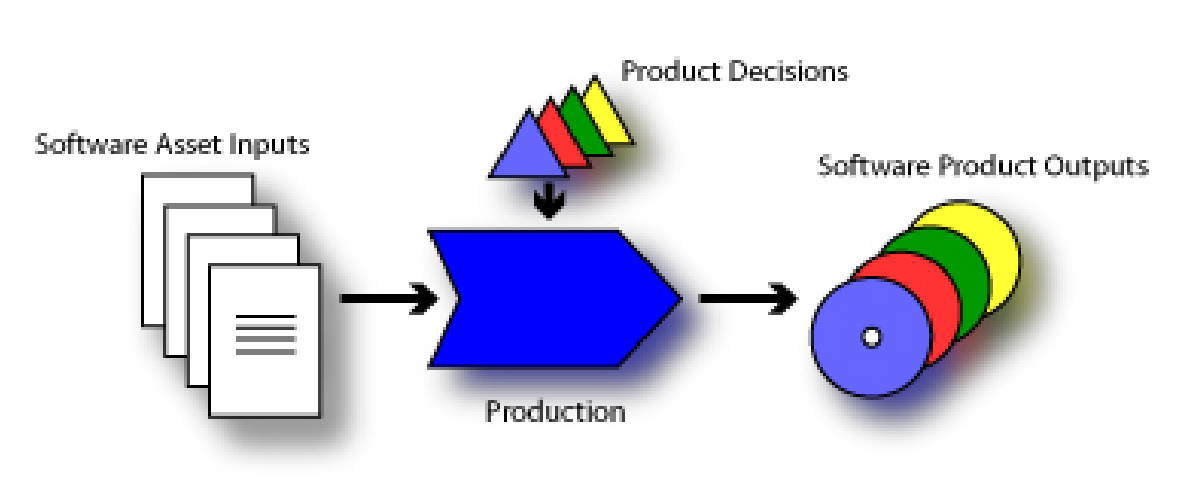
\includegraphics[scale=0.25]{img/spl.eps}
}

\end{frame}

\begin{frame}
\frametitle{Thesis context}

\begin{block}{Variability Management Problem}
\begin{itemize}
	\item Variable features often require variation points to be scattered trough
	different places in requirements, design, code, and test artifacts.
	\item As a consequence, it is painful to evolve a product line if it does not 
	exist a clear separation between variability concern and domain concerns.
\end{itemize}
\end{block}

\end{frame}

\begin{frame}
\frametitle{Thesis context}

\begin{block}{Hypothesis}
A better separation between VM and software engineering
artifacts improve:

\begin{itemize}
  \item SPL Evolvability
  \item SPL Traceability
  \item SPL Configurability
\end{itemize}
\end{block}

\begin{block}{Proposed approach:}
Improve this SoC by means of representing Variability Management as
crosscutting mechanisms.
\end{block}
\end{frame}

\begin{frame}
\frametitle{Thesis context}

\begin{block}{VM as crosscutting mechanisms}
Different input models crosscut each other with respect to a SPL member
(adapted from Masuhara and Kiczales - ECOOP 2003).
\end{block}
\onslide+<2>
\begin{block}{Big picture:}
\center{
 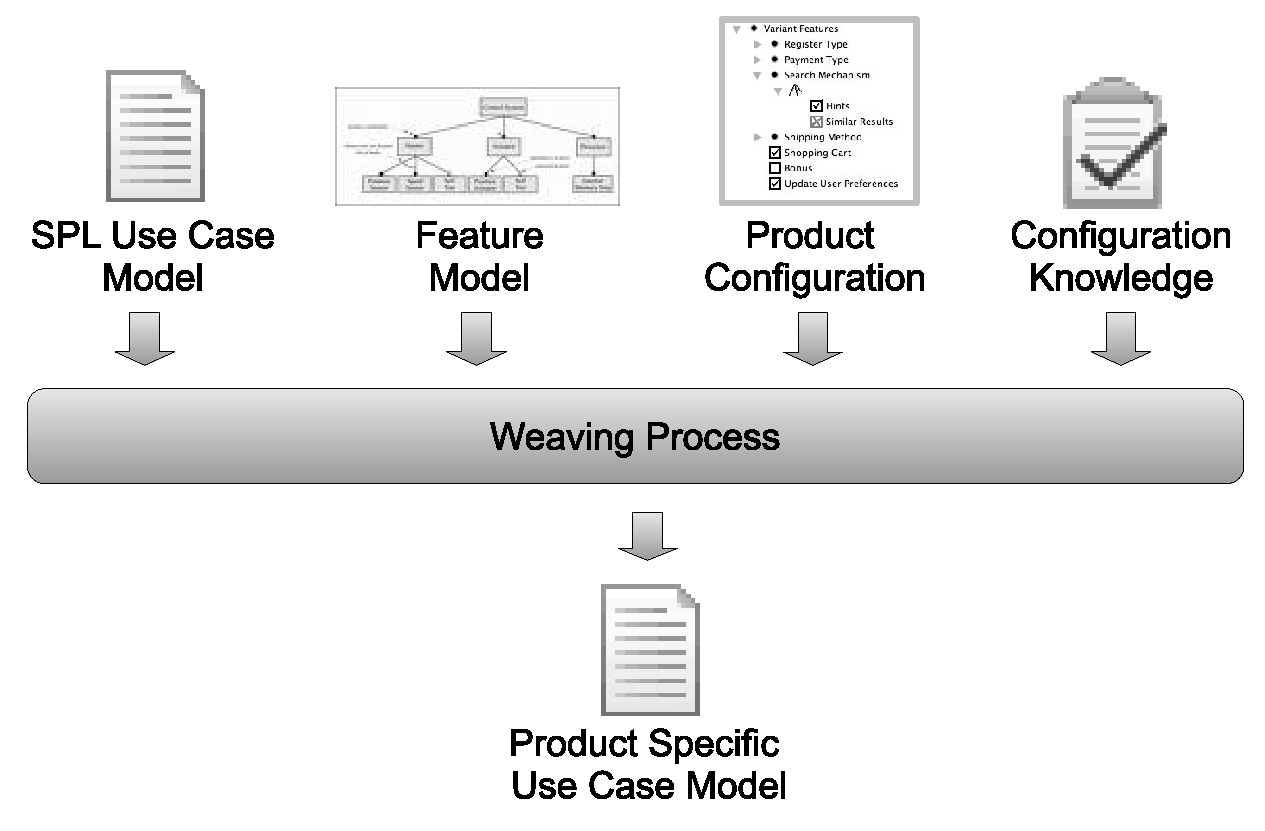
\includegraphics[scale=0.25]{img/weave-process2.eps}
}
\end{block}

\end{frame}

\begin{frame}
\frametitle{Thesis context}
\begin{block}{Weaving Process}
\begin{itemize}
  \hilite<1> \item sequence of weavers, guided by the
  configuration knowledge, that should be applied in order to generate specific instances.
  \hilite<2> \item Each weaver is represented as a tuple, which highlights the
  contribution of the corresponding input languages.
  \hilite<3> \item by relating the tuple elements to a reference
  implementation of the weaver.
\end{itemize}	
\end{block}


\end{frame}

\end{document}
